%************************************************
\chapter{Analisi dei requisiti}\label{ch:requisiti}
%************************************************
Il seguente capitolo descrive le caratteristiche principali che l'azienda \myCompany richiede vengano implementate nei prototipi: dopo una descrizione generale vengono descritti i casi d'uso rilevati e i requisiti che ne derivano.

I casi d'uso utilizzati per la progettazione dei prototipi hanno un codice identificativo univoco, nella forma:
\begin{center}
UC[codice univoco del padre].[codice progressivo di livello]
\end{center}
Il codice progressivo di livello può includere diversi livelli di gerarchia separati da un punto.

I requisiti vengono individuati dall'analisi effettuata sulle richieste dell'azienda, oppure emergono dai casi d'uso o nascono da esigenze interne; sono classificati per tipo e importanza secondo la seguente codifica:
\begin{center}
R[importanza][tipo][codice]
\end{center}

\begin{description}
\item[importanza:] \hfill 
	\begin{enumerate}
	\setcounter{enumi}{-1}
	\item Requisito obbligatorio;
	\item Requisito desiderabile;
	\item Requisito opzionale.
	\end{enumerate}
\item[tipo:] \hfill 
	\begin{description}
	\item[F:] Funzionale;
	\item[Q:] Di qualità;
	\item[P:] Prestazionale;
	\item[V:] Di vincolo.
	\end{description}
\item[codice:] è il codice univoco di ogni requisito espresso in modo gerarchico.
\end{description}

\section{MyNotes}
\subsection{Descrizione generale}
Lo scopo del prototipo è  l'implementazione del \emph{SyncEngine} per sviluppare un sistema di gestione note ed autori che sia in grado di lavorare offline e di sincronizzarsi con un server non appena si renda disponibile una connessione internet.

Il componente è già esistente e verranno quindi presentati i casi d'uso e i relativi requisiti solo per l'applicazione che lo deve utilizzare.

\subsection{Casi d'uso}
Vengono ora descritti i casi d'uso utilizzati per la progettazione del prototipo \emph{MyNotes}.

\subsubsection{Caso d'uso UC1: Scenario principale}
\begin{figure}[htb]
\centering
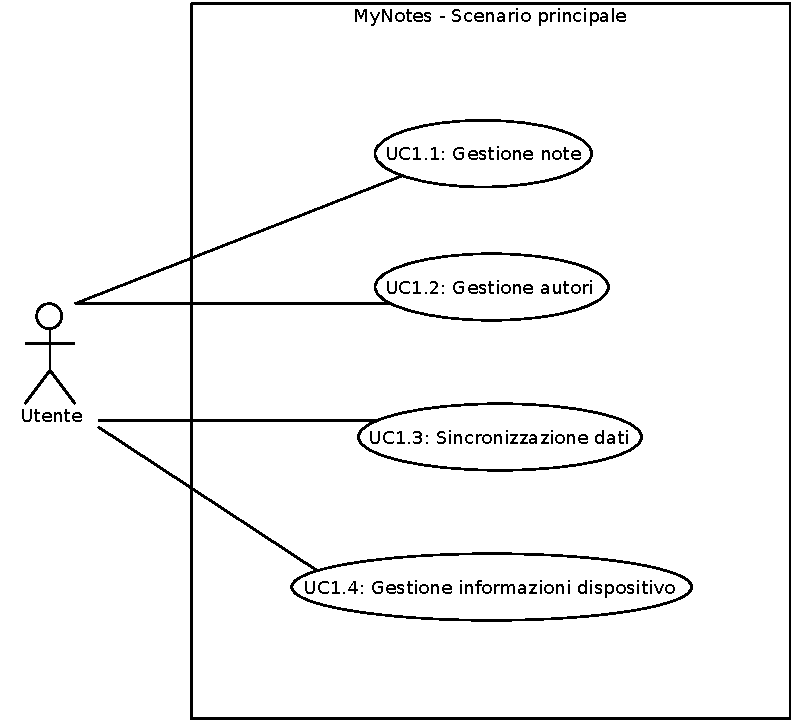
\includegraphics[scale=0.6]{gfx/useCase/MN_UC1_Scenario_principale.pdf}
\caption{Caso d'uso UC1: Scenario principale}
\label{fig:My notes UC1}
\end{figure}

\begin{description}
\item[attori:] Utente;
\item[scopo e descrizione:] L'utente ha avviato correttamente l'applicazione e questa è pronta all'uso. Egli può effettuare varie operazioni: eseguire la gestione delle note, degli autori e delle informazioni del dispositivo e sincronizzare i dati con il server remoto;
\item[precondizione:] L'applicazione è stata avviata ed è pronta all'uso.
\item[flusso principale degli eventi:] \hfill 
	\begin{enumerate}
	\item L'utente può eseguire la gestione delle note;
	\item L'utente può eseguire la gestione degli autori;
	\item L'utente può sincronizzare i dati con il server;
	\item L'utente può eseguire la gestione delle informazioni del dispositivo;
	\end{enumerate}
\item[postcondizione:] Il sistema ha ottenuto informazioni sulle operazioni che l'utente vuole eseguire.
\end{description}

\subsubsection{Caso d'uso UC1.1: Gestione note}
\begin{figure}[htb]
\centering
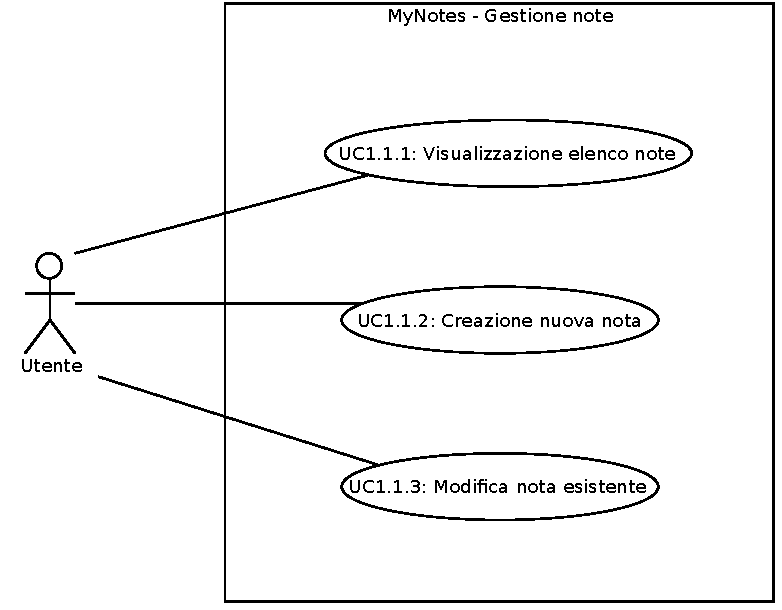
\includegraphics[scale=0.6]{gfx/useCase/MN_UC1-1_Gestione_note.pdf}
\caption{Caso d'uso UC1.1: Gestione note}
\label{fig:My notes UC1.1}
\end{figure}

\begin{description}
\item[attori:] Utente;
\item[scopo e descrizione:] L'utente desidera eseguire la gestione delle note;
\item[precondizione:] Il sistema è pronto a gestire le note;
\item[flusso principale degli eventi:] \hfill 
	\begin{enumerate}
	\item L'utente può visualizzare l'elenco delle note presenti nel dispositivo;
	\item L'utente può creare una nuova nota;
	\item L'utente può modificare una nota esistente;
	\end{enumerate}
\item[postcondizione:] Il sistema ha ottenuto informazioni sulle operazioni che l'utente vuole eseguire.
\end{description}

\subsubsection{Caso d'uso UC1.1.1: Visualizzazione elenco note}
\begin{description}
\item[attori:] Utente;
\item[scopo e descrizione:] L'utente desidera visualizzare l'elenco delle note esistenti;
\item[precondizione:] Il sistema è pronto a visualizzare le note;
\item[postcondizione:] Il sistema ha visualizzato le note esistenti.
\end{description}

\subsubsection{Caso d'uso UC1.1.2: Creazione nuova nota}
\begin{figure}[htb]
\centering
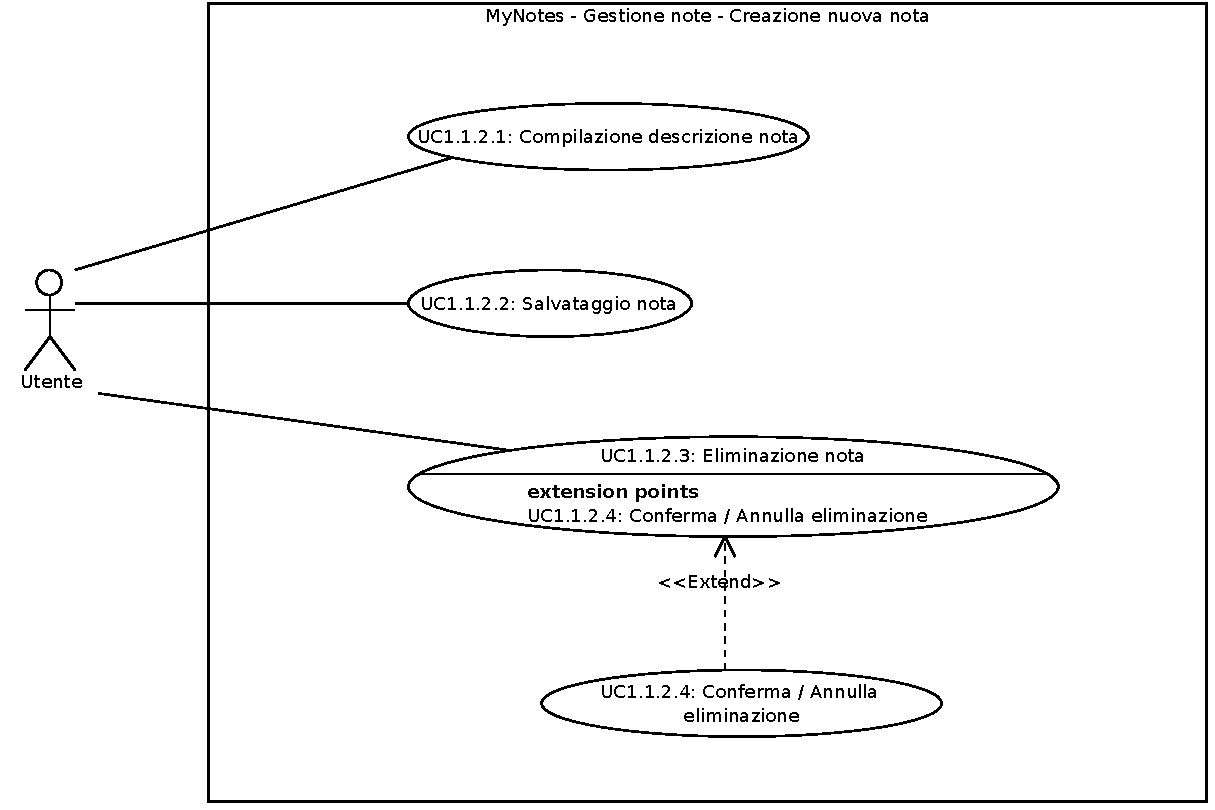
\includegraphics[scale=0.5]{gfx/useCase/MN_UC1-1-2_Creazione_nuova_nota.pdf}
\caption{Caso d'uso UC1.1.2: Creazione nuova nota}
\label{fig:My notes UC1.1.2}
\end{figure}

\begin{description}
\item[attori:] Utente;
\item[scopo e descrizione:] L'utente desidera creare una nuova nota;
\item[precondizione:] Il sistema è pronto alla creazione di una nuova nota;
\item[flusso principale degli eventi:] \hfill 
	\begin{enumerate}
	\item L'utente può compilare la descrizione della nota;
	\item L'utente può salvare la nota;
	\item L'utente può eliminare la nota;
	\end{enumerate}
\item[estensioni:] \hfill
	\begin{enumerate}
	\item Solo nel caso che l'utente desideri eliminare la nota corrente gli viene richiesta la conferma o l'annullamento dell'azione;
	\end{enumerate}
\item[postcondizione:] Il sistema ha eseguito il salvataggio della nuova nota o la cancellazione della stessa.
\end{description}

\subsubsection{Caso d'uso UC1.1.2.1: Compilazione descrizione nota}
\begin{description}
\item[attori:] Utente;
\item[scopo e descrizione:] L'utente desidera compilare la descrizione di una nuova nota;
\item[precondizione:] Il sistema ha generato una nuova nota, la visualizza ed è pronto alla sua compilazione;
\item[postcondizione:] Il sistema visualizza la descrizione inserita dall'utente ed è pronto al salvataggio o alla cancellazione.
\end{description}

\subsubsection{Caso d'uso UC1.1.2.2: Salvataggio nota}
\begin{description}
\item[attori:] Utente;
\item[scopo e descrizione:] L'utente desidera salvare la nuova nota;
\item[precondizione:] Il sistema visualizza la descrizione inserita dall'utente ed è pronto al salvataggio;
\item[postcondizione:] Il sistema ha eseguito correttamente il salvataggio della nuova nota.
\end{description}

\subsubsection{Caso d'uso UC1.1.2.3: Eliminazione nota}
\begin{description}
\item[attori:] Utente;
\item[scopo e descrizione:] L'utente desidera eliminare la nuova nota;
\item[precondizione:] Il sistema visualizza la descrizione inserita dall'utente ed è pronto alla cancellazione;
\item[postcondizione:] Il sistema ha eseguito correttamente l'eliminazione della nuova nota.
\end{description}

\subsubsection{Caso d'uso UC1.1.2.4: Conferma / Annulla eliminazione}
\begin{figure}[htb]
\centering
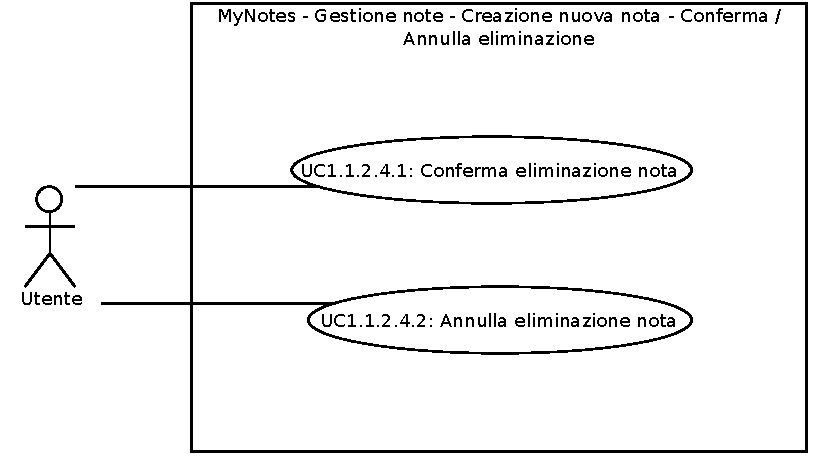
\includegraphics[scale=0.6]{gfx/useCase/MN_UC1-1-2-4_Conferma-Annulla_eliminazione.pdf}
\caption{Caso d'uso UC1.1.2.4: Conferma - Annulla eliminazione}
\label{fig:My notes UC1.1.2.4}
\end{figure}

\begin{description}
\item[attori:] Utente;
\item[scopo e descrizione:] L'utente desidera eliminare la nuova nota;
\item[precondizione:] Il sistema visualizza la descrizione inserita dall'utente ed è pronto alla cancellazione;
\item[flusso principale degli eventi:] \hfill
	\begin{enumerate}
	\item L'utente può confermare l'eliminazione della nota;
	\item L'utente può annullare l'eliminazione della nota;
	\end{enumerate}
\item[postcondizione:] Il sistema ha eseguito correttamente l'eliminazione della nuova nota o l'annullamento dell'operazione.
\end{description}

\subsubsection{Caso d'uso UC1.1.2.4.1: Conferma eliminazione nota}
\begin{description}
\item[attori:] Utente;
\item[scopo e descrizione:] L'utente desidera confermare l'eliminazione della nota;
\item[precondizione:] Il sistema chiede conferma dell'eliminazione della nota;
\item[postcondizione:] Il sistema ha eseguito correttamente l'eliminazione della nuova nota.
\end{description}

\subsubsection{Caso d'uso UC1.1.2.4.2: Annulla eliminazione nota}
\begin{description}
\item[attori:] Utente;
\item[scopo e descrizione:] L'utente desidera annullare l'eliminazione della nota;
\item[precondizione:] Il sistema chiede conferma dell'eliminazione della nota;
\item[postcondizione:] Il sistema ha eseguito correttamente l'annullamento dell'eliminazione della nuova nota.
\end{description}

\subsubsection{Caso d'uso UC1.1.3: Modifica nota esistente}
\begin{figure}[htb]
\centering
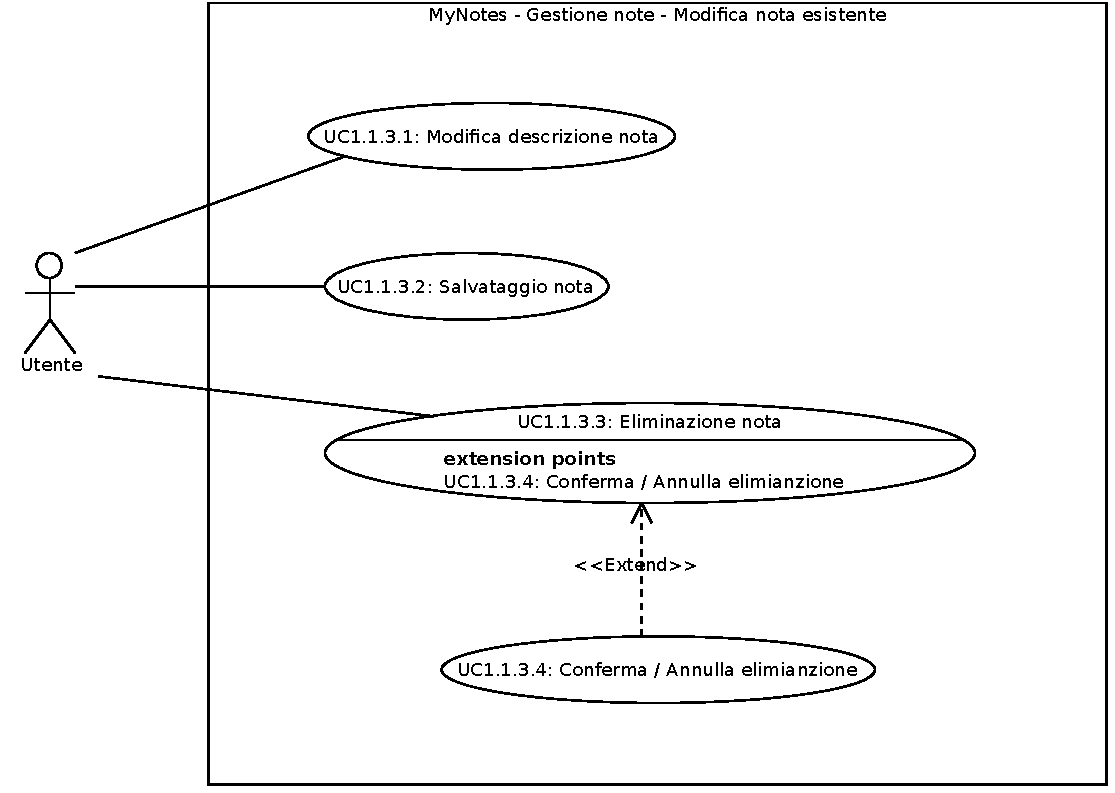
\includegraphics[scale=0.5]{gfx/useCase/MN_UC1-1-3_Modifica_nota_esistente.pdf}
\caption{Caso d'uso UC1.1.3: Modifica nota esistente}
\label{fig:My notes UC1.1.3}
\end{figure}

\begin{description}
\item[attori:] Utente;
\item[scopo e descrizione:] L'utente desidera modificare una nota esistente;
\item[precondizione:] Il sistema visualizza la nota da modificare.
\item[flusso principale degli eventi:] \hfill 
	\begin{enumerate}
	\item L'utente può modificare la descrizione della nota;
	\item L'utente può salvare la nota;
	\item L'utente può eliminare la nota;
	\end{enumerate}
\item[estensioni:] \hfill
	\begin{enumerate}
	\item Solo nel caso che l'utente desideri eliminare la nota corrente gli viene richiesta la conferma o l'annullamento dell'azione;
	\end{enumerate}
\item[postcondizione:] Il sistema ha eseguito il salvataggio delle modifiche alla nota o la cancellazione della stessa.
\end{description}

\subsubsection{Caso d'uso UC1.1.3.1: Modifica descrizione nota}
\begin{description}
\item[attori:] Utente;
\item[scopo e descrizione:] L'utente desidera modificare la descrizione di una nota esistente;
\item[precondizione:] Il sistema visualizza la nota ed è pronto alla sua modifica;
\item[postcondizione:] Il sistema visualizza la descrizione modificata dall'utente ed è pronto al salvataggio o alla cancellazione.
\end{description}

\subsubsection{Caso d'uso UC1.1.3.2: Salvataggio nota}
\begin{description}
\item[attori:] Utente;
\item[scopo e descrizione:] L'utente desidera salvare le modifiche alla nota;
\item[precondizione:] Il sistema visualizza la descrizione modificata dall'utente ed è pronto al salvataggio;
\item[postcondizione:] Il sistema ha eseguito correttamente il salvataggio della nota modificata.
\end{description}

\subsubsection{Caso d'uso UC1.1.3.3: Eliminazione nota}
\begin{description}
\item[attori:] Utente;
\item[scopo e descrizione:] L'utente desidera eliminare una nota esistente;
\item[precondizione:] Il sistema visualizza la descrizione della nota ed è pronto alla cancellazione;
\item[postcondizione:] Il sistema ha eseguito correttamente l'eliminazione della nota esistente.
\end{description}

\subsubsection{Caso d'uso UC1.1.3.4: Conferma / Annulla eliminazione}
\begin{figure}[htb]
\centering
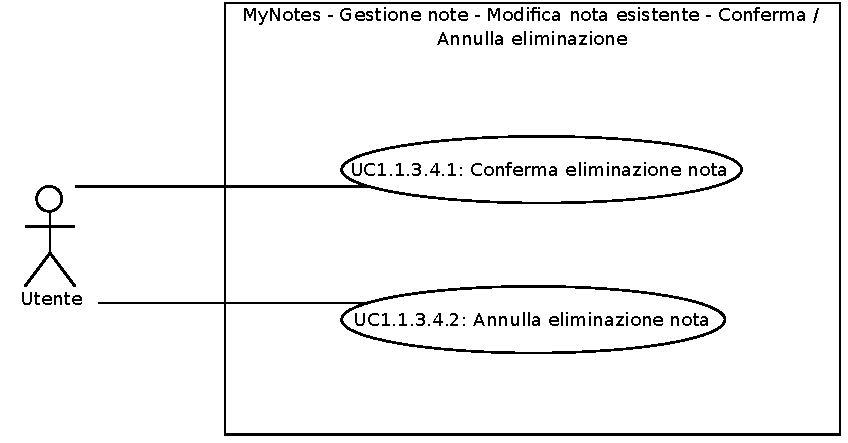
\includegraphics[scale=0.6]{gfx/useCase/MN_UC1-1-3-4_Conferma-Annulla_eliminazione.pdf}
\caption{Caso d'uso UC1.1.3.4: Conferma - Annulla eliminazione}
\label{fig:My notes UC1.1.3.4}
\end{figure}

\begin{description}
\item[attori:] Utente;
\item[scopo e descrizione:] L'utente desidera eliminare una nota esistente;
\item[precondizione:] Il sistema visualizza la descrizione della nota ed è pronto alla cancellazione;
\item[flusso principale degli eventi:] \hfill
	\begin{enumerate}
	\item L'utente può confermare l'eliminazione della nota;
	\item L'utente può annullare l'eliminazione della nota;
	\end{enumerate}
\item[postcondizione:] Il sistema ha eseguito correttamente l'eliminazione della nota o l'annullamento dell'operazione.
\end{description}

\subsubsection{Caso d'uso UC1.1.3.4.1: Conferma eliminazione nota}
\begin{description}
\item[attori:] Utente;
\item[scopo e descrizione:] L'utente desidera confermare l'eliminazione della nota;
\item[precondizione:] Il sistema chiede conferma dell'eliminazione della nota;
\item[postcondizione:] Il sistema ha eseguito correttamente l'eliminazione della nota.
\end{description}

\subsubsection{Caso d'uso UC1.1.3.4.2: Annulla eliminazione nota}
\begin{description}
\item[attori:] Utente;
\item[scopo e descrizione:] L'utente desidera annullare l'eliminazione della nota;
\item[precondizione:] Il sistema chiede conferma dell'eliminazione della nota;
\item[postcondizione:] Il sistema ha eseguito correttamente l'annullamento dell'eliminazione della nota.
\end{description}

\subsubsection{Caso d'uso UC1.2: Gestione autori}
\begin{figure}[htb]
\centering
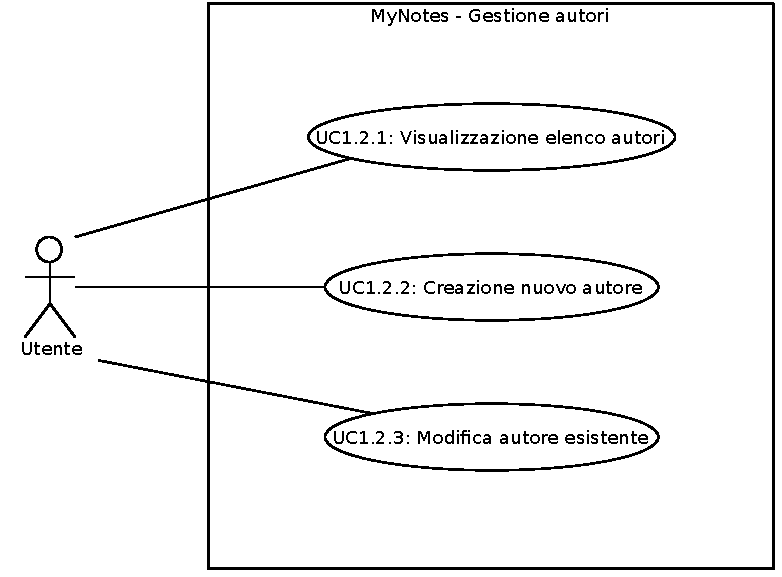
\includegraphics[scale=0.6]{gfx/useCase/MN_UC1-2_Gestione_autori.pdf}
\caption{Caso d'uso UC1.2: Gestione autori}
\label{fig:My notes UC1.2}
\end{figure}

\begin{description}
\item[attori:] Utente;
\item[scopo e descrizione:] L'utente desidera eseguire la gestione degli autori;
\item[precondizione:] Il sistema è pronto a gestire gli autori.
\item[flusso principale degli eventi:] \hfill 
	\begin{enumerate}
	\item L'utente può visualizzare l'elenco degli autori presenti nel dispositivo;
	\item L'utente può creare un nuovo autore;
	\item L'utente può modificare un autore esistente;
	\end{enumerate}
\item[postcondizione:] Il sistema ha ottenuto informazioni sulle operazioni che l'utente vuole eseguire.
\end{description}

\subsubsection{Caso d'uso UC1.2.1: Visualizzazione elenco autori}
\begin{description}
\item[attori:] Utente;
\item[scopo e descrizione:] L'utente desidera visualizzare l'elenco degli autori esistenti;
\item[precondizione:] Il sistema è pronto a visualizzare gli autori.
\item[postcondizione:] Il sistema ha visualizzato gli autori esistenti.
\end{description}

\subsubsection{Caso d'uso UC1.2.2: Creazione nuovo autore}
\begin{figure}[htb]
\centering
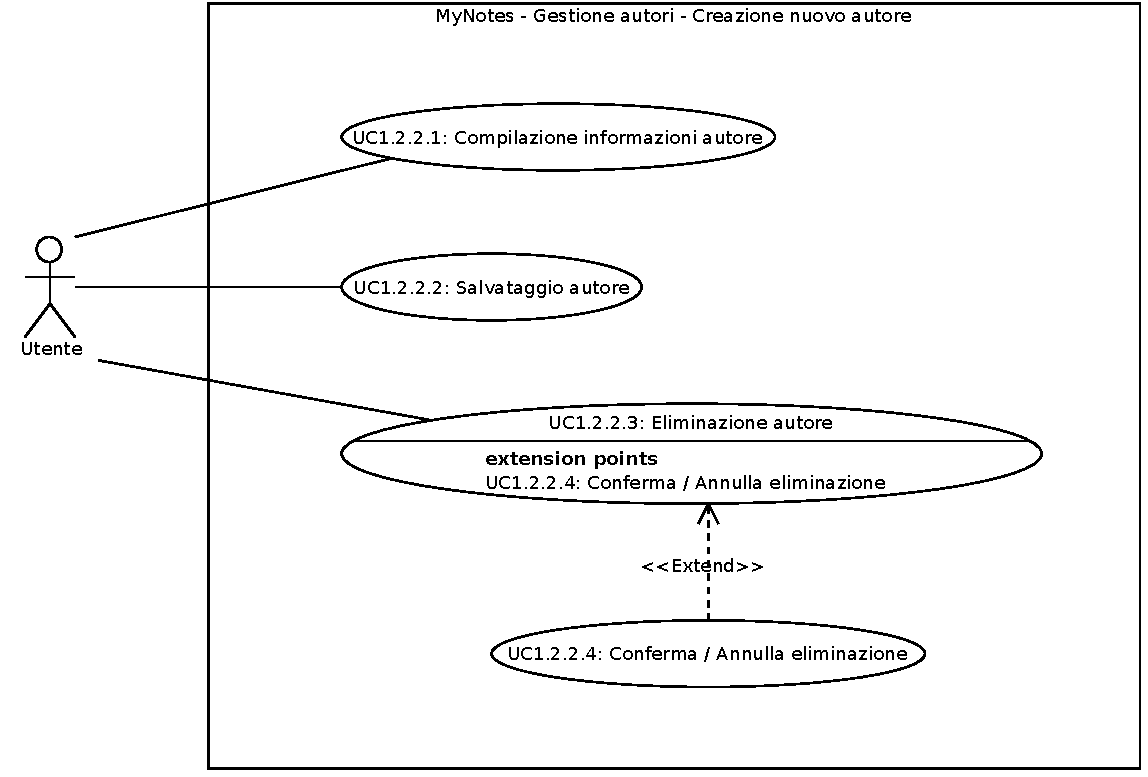
\includegraphics[scale=0.5]{gfx/useCase/MN_UC1-2-2_Creazione_nuovo_autore.pdf}
\caption{Caso d'uso UC1.2.2: Creazione nuovo autore}
\label{fig:My notes UC1.2.2}
\end{figure}

\begin{description}
\item[attori:] Utente;
\item[scopo e descrizione:] L'utente desidera creare un nuovo autore;
\item[precondizione:] Il sistema è pronto alla creazione di un nuovo autore.
\item[flusso principale degli eventi:] \hfill 
	\begin{enumerate}
	\item L'utente può compilare le informazioni dell'autore;
	\item L'utente può salvare l'autore;
	\item L'utente può eliminare l'autore;
	\end{enumerate}
\item[estensioni:] \hfill
	\begin{enumerate}
	\item Solo nel caso che l'utente desideri eliminare l'autore corrente gli viene richiesta la conferma o l'annullamento dell'azione;
	\end{enumerate}
\item[postcondizione:] Il sistema ha eseguito il salvataggio del nuovo autore o la cancellazione dello stesso.
\end{description}

\subsubsection{Caso d'uso UC1.2.2.1: Compilazione informazioni autore}
\begin{description}
\item[attori:] Utente;
\item[scopo e descrizione:] L'utente desidera compilare le informazioni di un nuovo autore;
\item[precondizione:] Il sistema ha generato un nuovo autore, lo visualizza ed è pronto alla sua compilazione;
\item[postcondizione:] Il sistema visualizza le informazioni inserite dall'utente ed è pronto al salvataggio o alla cancellazione.
\end{description}

\subsubsection{Caso d'uso UC1.2.2.2: Salvataggio autore}
\begin{description}
\item[attori:] Utente;
\item[scopo e descrizione:] L'utente desidera salvare il nuovo autore;
\item[precondizione:] Il sistema visualizza le informazioni inserite dall'utente ed è pronto al salvataggio;
\item[postcondizione:] Il sistema ha eseguito correttamente il salvataggio del nuovo autore.
\end{description}

\subsubsection{Caso d'uso UC1.2.2.3: Eliminazione autore}
\begin{description}
\item[attori:] Utente;
\item[scopo e descrizione:] L'utente desidera eliminare il nuovo autore;
\item[precondizione:] Il sistema visualizza le informazioni inserite dall'utente ed è pronto alla cancellazione;
\item[postcondizione:] Il sistema ha eseguito correttamente l'eliminazione del nuovo autore.
\end{description}

\subsubsection{Caso d'uso UC1.2.2.4: Conferma / Annulla eliminazione}
\begin{figure}[htb]
\centering
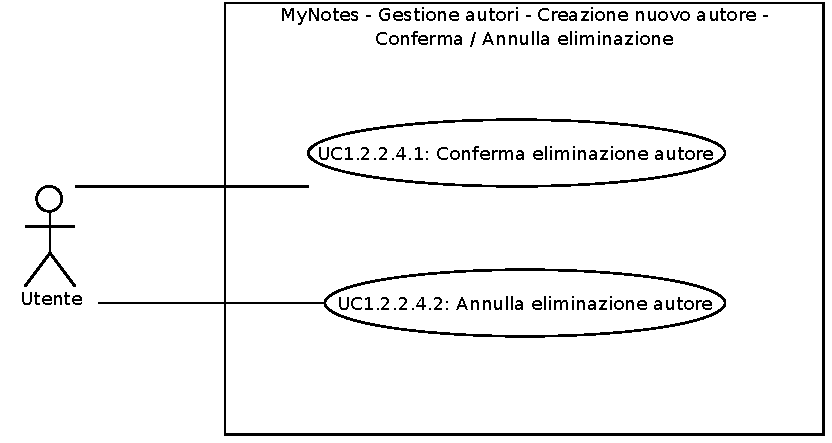
\includegraphics[scale=0.6]{gfx/useCase/MN_UC1-2-2-4_Conferma-Annulla_eliminazione.pdf}
\caption{Caso d'uso UC1.2.2.4: Conferma - Annulla eliminazione}
\label{fig:My notes UC1.2.2.4}
\end{figure}

\begin{description}
\item[attori:] Utente;
\item[scopo e descrizione:] L'utente desidera eliminare il nuovo autore;
\item[precondizione:] Il sistema visualizza le informazioni inserite dall'utente ed è pronto alla cancellazione;
\item[flusso principale degli eventi:] \hfill
	\begin{enumerate}
	\item L'utente può confermare l'eliminazione dell'autore;
	\item L'utente può annullare l'eliminazione dell'autore;
	\end{enumerate}
\item[postcondizione:] Il sistema ha eseguito correttamente l'eliminazione del nuovo autore o l'annullamento dell'operazione.
\end{description}

\subsubsection{Caso d'uso UC1.2.2.4.1: Conferma eliminazione autore}
\begin{description}
\item[attori:] Utente;
\item[scopo e descrizione:] L'utente desidera confermare l'eliminazione dell'autore;
\item[precondizione:] Il sistema chiede conferma dell'eliminazione dell'autore;
\item[postcondizione:] Il sistema ha eseguito correttamente l'eliminazione del nuovo autore.
\end{description}

\subsubsection{Caso d'uso UC1.2.2.4.2: Annulla eliminazione autore}
\begin{description}
\item[attori:] Utente;
\item[scopo e descrizione:] L'utente desidera annullare l'eliminazione dell'autore;
\item[precondizione:] Il sistema chiede conferma dell'eliminazione dell'autore;
\item[postcondizione:] Il sistema ha eseguito correttamente l'annullamento dell'eliminazione del nuovo autore.
\end{description}

\subsubsection{Caso d'uso UC1.2.3: Modifica autore esistente}
\begin{figure}[htb]
\centering
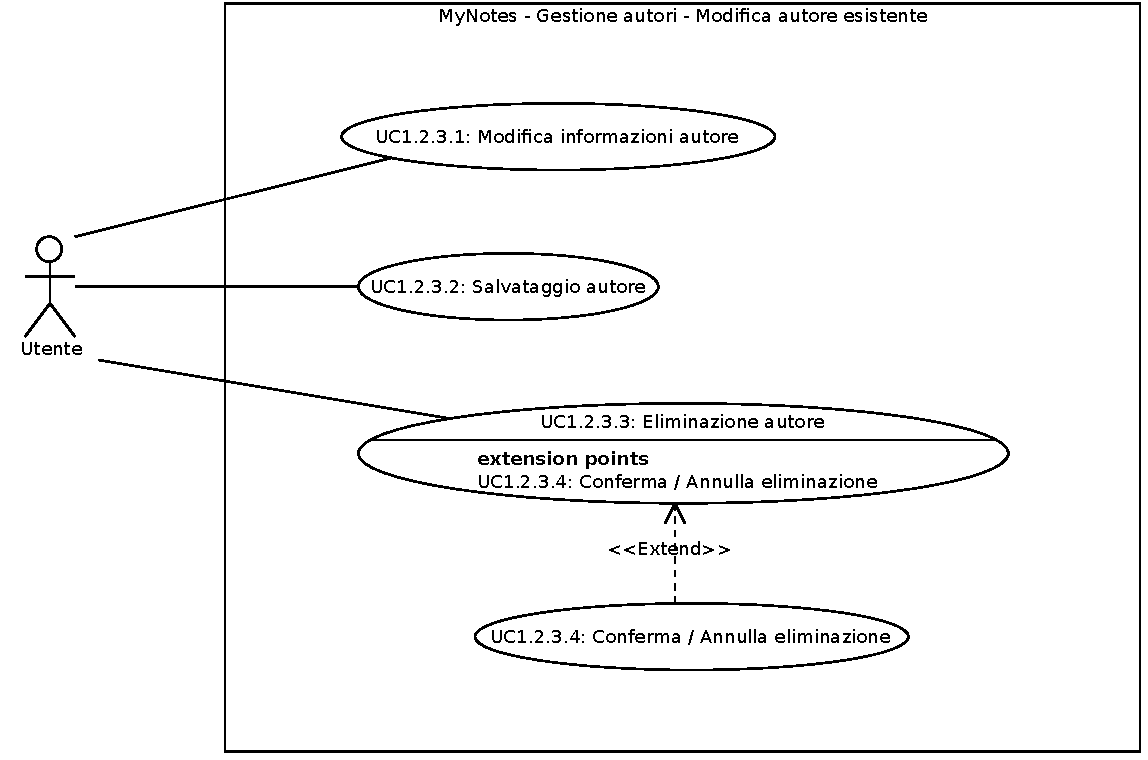
\includegraphics[scale=0.5]{gfx/useCase/MN_UC1-2-3_Modifica_autore_esistente.pdf}
\caption{Caso d'uso UC1.2.3: Modifica autore esistente}
\label{fig:My notes UC1.2.3}
\end{figure}

\begin{description}
\item[attori:] Utente;
\item[scopo e descrizione:] L'utente desidera modificare un autore esistente;
\item[precondizione:] Il sistema visualizza l'autore da modificare.
\item[flusso principale degli eventi:] \hfill 
	\begin{enumerate}
	\item L'utente può modificare le informazioni dell'autore;
	\item L'utente può salvare l'autore;
	\item L'utente può eliminare l'autore;
	\end{enumerate}
\item[estensioni:] \hfill
	\begin{enumerate}
	\item Solo nel caso che l'utente desideri eliminare l'autore corrente gli viene richiesta la conferma o l'annullamento dell'azione;
	\end{enumerate}
\item[postcondizione:] Il sistema ha eseguito il salvataggio delle modifiche all'autore o la cancellazione dello stesso.
\end{description}

\subsubsection{Caso d'uso UC1.2.3.1: Modifica informazioni autore}
\begin{description}
\item[attori:] Utente;
\item[scopo e descrizione:] L'utente desidera modificare le informazioni di un autore esistente;
\item[precondizione:] Il sistema visualizza un autore esistente ed è pronto alla sua modifica;
\item[postcondizione:] Il sistema visualizza le informazioni modificate dall'utente ed è pronto al salvataggio o alla cancellazione.
\end{description}

\subsubsection{Caso d'uso UC1.2.3.2: Salvataggio autore}
\begin{description}
\item[attori:] Utente;
\item[scopo e descrizione:] L'utente desidera salvare le modifiche all'autore;
\item[precondizione:] Il sistema visualizza le informazioni modificate dall'utente ed è pronto al salvataggio;
\item[postcondizione:] Il sistema ha eseguito correttamente il salvataggio dell'autore.
\end{description}

\subsubsection{Caso d'uso UC1.2.3.3: Eliminazione autore}
\begin{description}
\item[attori:] Utente;
\item[scopo e descrizione:] L'utente desidera eliminare un autore esistente;
\item[precondizione:] Il sistema visualizza le informazioni dell'autore ed è pronto alla cancellazione;
\item[postcondizione:] Il sistema ha eseguito correttamente l'eliminazione dell'autore.
\end{description}

\subsubsection{Caso d'uso UC1.2.3.4: Conferma / Annulla eliminazione}
\begin{figure}[htb]
\centering
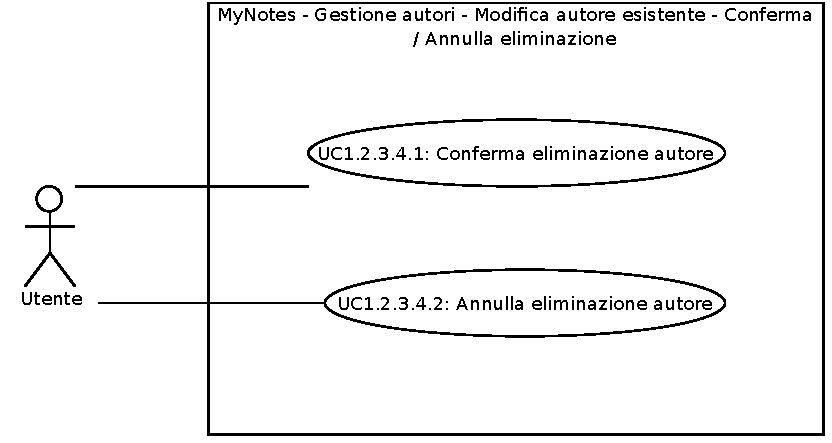
\includegraphics[scale=0.6]{gfx/useCase/MN_UC1-2-3-4_Conferma-Annulla_eliminazione.pdf}
\caption{Caso d'uso UC1.2.3.4: Conferma - Annulla eliminazione}
\label{fig:My notes UC1.2.3.4}
\end{figure}

\begin{description}
\item[attori:] Utente;
\item[scopo e descrizione:] L'utente desidera eliminare un autore esistente;
\item[precondizione:] Il sistema visualizza le informazioni dell'autore ed è pronto alla cancellazione;
\item[flusso principale degli eventi:] \hfill
	\begin{enumerate}
	\item L'utente può confermare l'eliminazione dell'autore;
	\item L'utente può annullare l'eliminazione dell'autore;
	\end{enumerate}
\item[postcondizione:] Il sistema ha eseguito correttamente l'eliminazione dell'autore esistente o l'annullamento dell'operazione.
\end{description}

\subsubsection{Caso d'uso UC1.2.3.4.1: Conferma eliminazione autore}
\begin{description}
\item[attori:] Utente;
\item[scopo e descrizione:] L'utente desidera confermare l'eliminazione dell'autore;
\item[precondizione:] Il sistema chiede conferma dell'eliminazione dell'autore;
\item[postcondizione:] Il sistema ha eseguito correttamente l'eliminazione dell'autore.
\end{description}

\subsubsection{Caso d'uso UC1.2.3.4.2: Annulla eliminazione autore}
\begin{description}
\item[attori:] Utente;
\item[scopo e descrizione:] L'utente desidera annullare l'eliminazione dell'autore;
\item[precondizione:] Il sistema chiede conferma dell'eliminazione dell'autore;
\item[postcondizione:] Il sistema ha eseguito correttamente l'annullamento dell'eliminazione dell'autore.
\end{description}

\subsubsection{Caso d'uso UC1.3: Sincronizzazione dati}
\begin{figure}[htb]
\centering
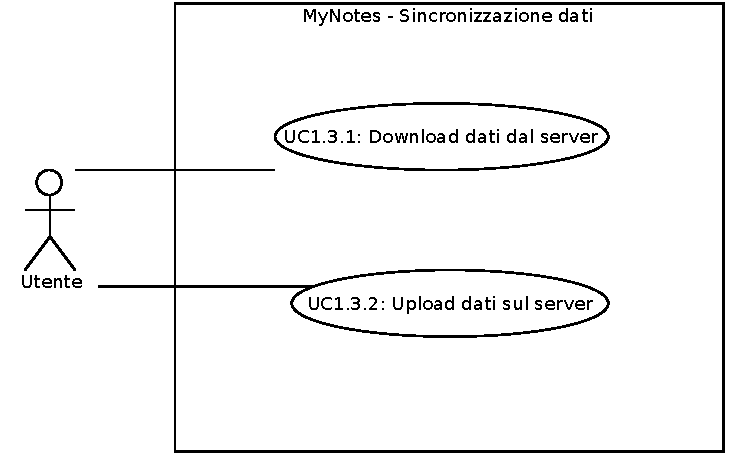
\includegraphics[scale=0.6]{gfx/useCase/MN_UC1-3_Sincronizzazione_dati.pdf}
\caption{Caso d'uso UC1.3: Sincronizzazione dati}
\label{fig:My notes UC1.3}
\end{figure}

\begin{description}
\item[attori:] Utente;
\item[scopo e descrizione:] L'utente desidera sincronizzare i dati con il server;
\item[precondizione:] Il sistema è pronto per la sincronizzazione dei dati; è presente una connessione internet.
\item[flusso principale degli eventi:] \hfill 
	\begin{enumerate}
	\item L'utente può effettuare il download dei dati presenti nel server;
	\item L'utente può effettuare l'upload nel server dei dati presenti nel dispositivo;
	\end{enumerate}
\item[postcondizione:] Il sistema ha ottenuto informazioni sulle operazioni che l'utente vuole eseguire.
\end{description}

\subsubsection{Caso d'uso UC1.3.1: Download dati dal server}
\begin{description}
\item[attori:] Utente;
\item[scopo e descrizione:] L'utente desidera scaricare i dati dal server;
\item[precondizione:] Il sistema è pronto per lo scaricamento dei dati; è presente una connessione internet.
\item[postcondizione:] Il sistema ha eseguito correttamente il download dei dati presenti nel server.
\end{description}

\subsubsection{Caso d'uso UC1.3.2: Upload dati sul server}
\begin{description}
\item[attori:] Utente;
\item[scopo e descrizione:] L'utente desidera caricare i dati sul server;
\item[precondizione:] Il sistema è pronto per il caricamento dei dati; è presente una connessione internet.
\item[postcondizione:] Il sistema ha eseguito correttamente l'upload nel server dei dati presenti nel dispositivo.
\end{description}

\subsubsection{Caso d'uso UC1.4: Gestione informazioni dispositivo}
\begin{figure}[htb]
\centering
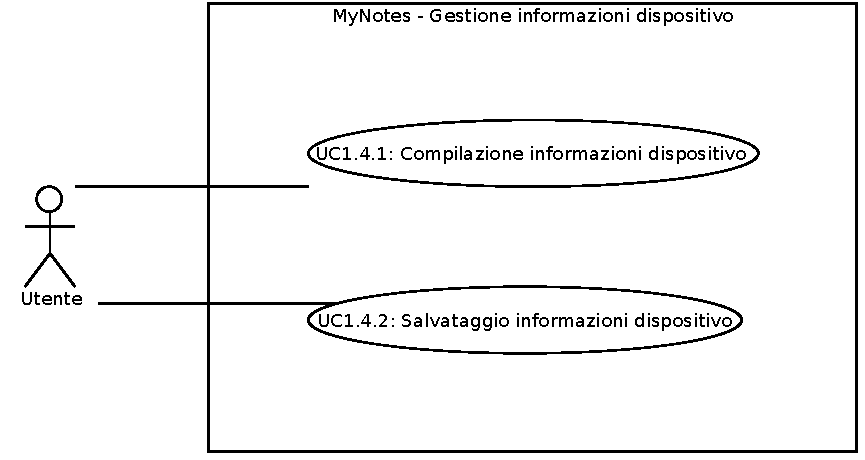
\includegraphics[scale=0.6]{gfx/useCase/MN_UC1-4_Gestione_informazioni_dispositivo.pdf}
\caption{Caso d'uso UC1.4: Gestione informazioni dispositivo}
\label{fig:My notes UC1.4}
\end{figure}

\begin{description}
\item[attori:] Utente;
\item[scopo e descrizione:] L'utente desidera gestire le informazioni del dispositivo;
\item[precondizione:] Il sistema è pronto per la gestione delle informazioni del dispositivo;
\item[flusso principale degli eventi:] \hfill 
	\begin{enumerate}
	\item L'utente può compilare le informazioni del dispositivo;
	\item L'utente può salvare le informazioni del dispositivo;
	\end{enumerate}
\item[postcondizione:] Il sistema ha ottenuto informazioni sulle operazioni che l'utente vuole eseguire.
\end{description}

\subsubsection{Caso d'uso UC1.4.1: Compilazione informazioni dispositivo}
\begin{description}
\item[attori:] Utente;
\item[scopo e descrizione:] L'utente desidera compilare le informazioni del dispositivo;
\item[precondizione:] Il sistema visualizza la scheda delle informazioni del dispositivo pronta per essere compilata;
\item[postcondizione:] Il sistema visualizza le informazioni inserite dall'utente ed è pronto al salvataggio.
\end{description}

\subsubsection{Caso d'uso UC1.4.2: Salvataggio informazioni dispositivo}
\begin{description}
\item[attori:] Utente;
\item[scopo e descrizione:] L'utente desidera salvare le informazioni del dispositivo;
\item[precondizione:] Il sistema è pronto per il salvataggio delle informazioni del dispositivo;
\item[postcondizione:] Il sistema ha eseguito correttamente il salvataggio delle informazioni dispositivo.
\end{description}

\subsection{Requisiti}
Vengono ora descritti i requisiti suddivisi per tipologia.

\subsubsection{Requisiti funzionali}
Di seguito viene riportata la tabella che esprime i requisiti funzionali.
%**************************************
%    tabella requisiti funzionali
%**************************************
\rowcolors{1}{lightCyan}{paleTurquoise}
\begin{longtable}{lp{0.60\textwidth}l}
\hiderowcolors
\caption{Requisiti funzionali -- MyNotes}
\label{tab:requsiti funzionali MyNotes} \\
%intestazione iniziale
\toprule \hiderowcolors
Codice & Descrizione & Fonte \\
\midrule
\endfirsthead
%intestazione normale
\hiderowcolors
\multicolumn{3}{l}{\footnotesize\itshape Continua dalla pagina precedente}\\
\toprule \hiderowcolors
Codice & Descrizione & Fonte \\
\midrule
\endhead
%piede normale
\midrule \hiderowcolors
\multicolumn{3}{r}{\footnotesize\itshape Continua nella prossima pagina}\\
\endfoot
%piede finale
\bottomrule \hiderowcolors
\multicolumn{3}{r}{\footnotesize\itshape Si conclude dalla pagina precedente}\\
\endlastfoot
%corpo della tabella
\showrowcolors
%gestione nota
R0F1
& L'utente deve poter eseguire la gestione delle note
& UC1.1 \\
R0F1.1
& L'utente deve poter visualizzare l'elenco delle note
& UC1.1.1 \\
%nuova nota
R0F1.2
& L'utente deve poter creare una nuova nota
& UC1.1.2 \\
R0F1.2.1
& L'utente deve poter compilare la descrizione di una nuova nota
& UC1.1.2.1 \\
R0F1.2.2
& L'utente deve poter effettuare il salvataggio di una nuova nota
& UC1.1.2.2 \\
R0F1.2.3
& L'utente deve poter eliminare una nuova nota
& UC1.1.2.3 \\
R0F1.2.4
& L'utente deve poter confermare o annullare l'eliminazione di una nuova nota
& UC1.1.2.4 \\
R0F1.2.4.1
& L'utente deve poter confermare l'eliminazione di una nuova nota
& UC1.1.2.4.1 \\
R0F1.2.4.2
& L'utente deve poter annullare l'eliminazione di una nuova nota
& UC1.1.2.4.1 \\
%modifica nota
R0F1.3
& L'utente deve poter effettuare la modifica di una nota esistente
& UC1.1.3 \\
R0F1.3.1
& L'utente deve poter modificare la descrizione di una nota esistente
& UC1.1.3.1 \\
R0F1.3.2
& L'utente deve poter effettuare il salvataggio delle modifiche ad una nota esistente
& UC1.1.3.2 \\
R0F1.3.3
& L'utente deve poter effettuare l'eliminazione di una nota esistente
& UC1.1.3.3 \\
R0F1.3.4
& L'utente deve poter confermare o annullare l'eliminazione di una nota esistente
& UC1.1.3.4 \\
R0F1.3.4.1
& L'utente deve poter confermare l'eliminazione di una nota esistente
& UC1.1.3.4.1 \\
R0F1.3.4.2
& L'utente deve poter annullare l'eliminazione di una nota esistente
& UC1.1.3.4.1 \\
%gestione autori
R0F2
& L'utente deve poter eseguire la gestione degli autori
& UC1.2 \\
R0F2.1
& L'utente deve poter visualizzare l'elenco degli autori
& UC1.2.1 \\
%nuovo autore
R0F2.2
& L'utente deve poter effettuare la creazione di un nuovo autore
& UC1.2.2 \\
R0F2.2.1
& L'utente deve poter compilare la descrizione di un nuovo autore
& UC1.2.2.1 \\
R0F2.2.2
& L'utente deve poter effettuare il salvataggio di un nuovo autore
& UC1.2.2.2 \\
R0F2.2.3
& L'utente deve poter effettuare l'eliminazione di un nuovo autore
& UC1.2.2.3 \\
R0F2.2.4
& L'utente deve poter confermare o annullare l'eliminazione di un nuovo autore
& UC1.2.2.4 \\
R0F2.2.4.1
& L'utente deve poter confermare l'eliminazione di un nuovo autore
& UC1.2.2.4.1 \\
R0F2.2.4.2
& L'utente deve poter annullare l'eliminazione di un nuovo autore
& UC1.2.2.4.1 \\
%modifica autore
R0F2.3
& L'utente deve poter effettuare la modifica di un autore esistente
& UC1.2.3 \\
R0F2.3.1
& L'utente deve poter modificare la descrizione di un autore esistente
& UC1.2.3.1 \\
R0F2.3.2
& L'utente deve poter effettuare il salvataggio delle modifiche ad un autore esistente
& UC1.2.3.2 \\
R0F2.3.3
& L'utente deve poter effettuare l'eliminazione di un autore esistente
& UC1.2.3.3 \\
R0F2.3.4
& L'utente deve poter confermare o annullare l'eliminazione di un autore esistente
& UC1.2.3.4 \\
R0F2.3.4.1
& L'utente deve poter confermare l'eliminazione di un autore esistente
& UC1.2.3.4.1 \\
R0F2.3.4.2
& L'utente deve poter annullare l'eliminazione di un autore esistente
& UC1.2.3.4.2 \\
%sincronizzazione dati
R0F3
& L'utente deve poter effettuare la sincronizzazione dei dati con il server
& UC1.3 \\
R0F3.1
& L'utente deve poter effettuare il download dei dati dal server
& UC1.3.1 \\
R0F3.2
& L'utente deve poter effettuare l'upload dei dati sul server
& UC1.3.2 \\
%gestione info dispositivo
R0F4
& L'utente deve poter effettuare la gestione delle informazioni del dispositivo
& UC1.4 \\
R0F4.1
& L'utente deve poter compilare le informazioni del dispositivo
& UC1.4.1 \\
R0F4.2
& L'utente deve poter effettuare il salvataggio delle informazioni del dispositivo
& UC1.4.2 \\
R0F5
& L'applicazione deve fornire un'interfaccia utente grafica
& Capitolato \\
\end{longtable}

\subsubsection{Requisiti di vincolo}
Di seguito viene riportata la tabella che esprime i requisiti di vincolo.
%**************************************
%    tabella requisiti di vincolo
%**************************************
\begin{longtable}{lp{0.65\textwidth}l}
\caption{Tabella dei requisiti di vincolo}
\label{tab:requsiti vincolo} \\
%intestazione iniziale
\toprule
Codice & Descrizione & Fonte \\
\midrule
\endfirsthead
%intestazione normale
\multicolumn{3}{l}{\footnotesize\itshape Continua dalla pagina precedente}\\
\toprule
Codice & Descrizione & Fonte \\
\midrule
\endhead
%piede normale
\midrule
\multicolumn{3}{r}{\footnotesize\itshape Continua nella prossima pagina}\\
\endfoot
%piede finale
\bottomrule
\multicolumn{3}{r}{\footnotesize\itshape Si conclude dalla pagina precedente}\\
\endlastfoot
%corpo della tabella
R0V1 & L'applicazione deve essere funzionante su piattaforma Android 				& Capitolato \\[7mm]
R0V2 & L'applicazione deve essere funzionante su piattaforma iOS 					& Capitolato \\[7mm]
R0V3 & L'applicazione deve essere sviluppata con Sencha Touch 2 					& Capitolato \\[7mm]
R2V4 & L'applicazione deve essere sviluppata con Apache Cordova (Adobe PhoneGap) 	& Capitolato \\
\end{longtable}

%\subsection{Requisiti prestazionali}
%Di seguito viene riportata la tabella che esprime i requisiti prestazionali.
%%**************************************
%    tabella requisiti prestazionali
%**************************************

\subsubsection{Requisiti di qualità}
Di seguito viene riportata la tabella che esprime i requisiti di qualità.
%**************************************
%    tabella requisiti di qualità
%**************************************
\rowcolors{1}{lightCyan}{paleTurquoise}
\begin{longtable}{lp{0.65\textwidth}l}
\hiderowcolors
\caption{Requisiti di qualità - MyNotes}
\label{tab:requsiti qualità MyNotes} \\
%intestazione iniziale
\toprule \hiderowcolors
Codice & Descrizione & Fonte \\
\midrule
\endfirsthead
%intestazione normale
\hiderowcolors
\multicolumn{3}{l}{\footnotesize\itshape Continua dalla pagina precedente}\\
\toprule \hiderowcolors
Codice & Descrizione & Fonte \\
\midrule
\endhead
%piede normale
\midrule \hiderowcolors
\multicolumn{3}{r}{\footnotesize\itshape Continua nella prossima pagina}\\
\endfoot
%piede finale
\bottomrule %\hiderowcolors
%\multicolumn{3}{r}{\footnotesize\itshape Si conclude dalla pagina precedente}\\
\endlastfoot
%corpo della tabella
\showrowcolors
R0Q1 & Deve essere prodotta la documentazione del codice sorgente dell'applicazione 	 & Capitolato \\
R0Q2 & Deve essere prodotto un resoconto dettagliato dell'implementazione del SyncEngine & Capitolato \\
\end{longtable}

\section{SensorDevice}
\subsection{Descrizione generale}
L'obiettivo dell'azienda è studiare le possibili implementazioni delle librerie esistenti (\emph{Sencha Touch} e \emph{Apache Cordova}) per l'utilizzo dei sensori presenti nei device mobili con lo scopo di integrare tali caratteristiche in un prototipo dimostrativo funzionante su piattaforma Android e iOS.
Le funzionalità che risulteranno essere perfettamente funzionanti verranno integrate nell'applicativo che l'azienda sta sviluppando su richiesta di alcuni clienti.

Le funzionalità a cui l'azienda è interessata sono le seguenti:
\begin{itemize}
\item Scansione barcode;
\item Cattura immagini, video, registrazioni audio;
\item Lettura elenco contatti del dispositivo in uso;
\item Recupero informazioni proprie del dispositivo;
\item Backup e ripristino dei dati dell'applicazione sulla memoria di massa del dispositivo tramite un database \emph{SQLite} \cite{hipp:sqlite};
\item Geolocalizzazione.
\end{itemize}

Essendo tale applicazione un prototipo interno all'azienda non sono richiesti particolari vincoli di efficienza e un'interfaccia grafica accattivante: è stata lasciata libera iniziativa di sviluppare diverse soluzioni con l'obiettivo finale di ottenere un resoconto dettagliato dei risultati ottenuti.

\subsection{Casi d'uso}
Vengono ora descritti i casi d'uso utilizzati per la progettazione del prototipo \emph{SensorDevice}.

\subsubsection{Caso d'uso UC1: Scenario principale}
\begin{figure}[htb]
\centering
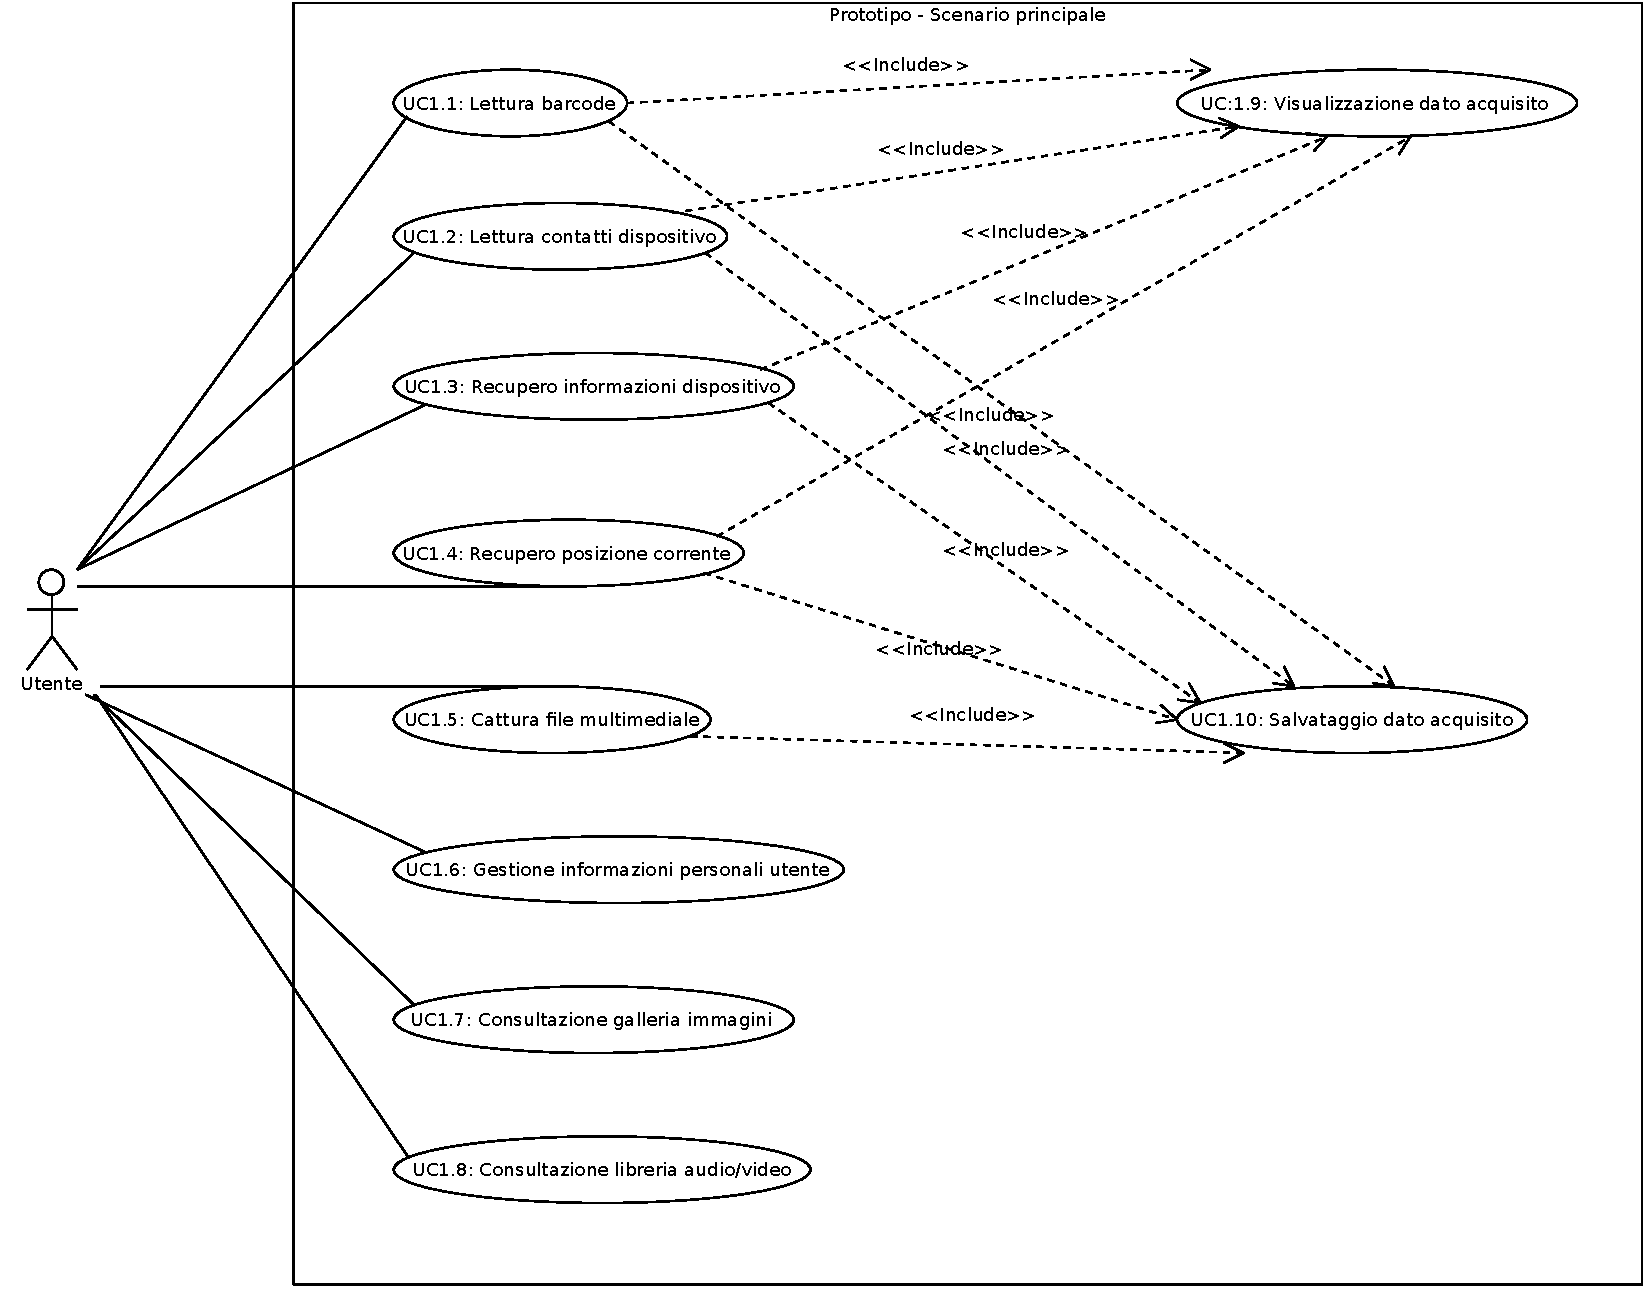
\includegraphics[scale=0.45]{gfx/useCase/UC1_Scenario_principale.pdf}
\caption{Caso d'uso UC1: Scenario principale}
\label{fig:UC1}
\end{figure}

\begin{description}
\item[attori:] Utente;
\item[scopo e descrizione:] L'utente ha avviato correttamente l'applicazione e questa è pronta all'uso. Egli può effettuare varie operazioni: leggere codici a barre, recuperare i contatti del dispositivo, recuperare le informazioni del dispositivo, catturare dati multimediali, recuperare la posizione corrente dal \ac{GPS}, gestire le proprie informazioni personali, consultare la galleria immagini e la libreria audio/video; il sistema provvederà a salvare correttamente tutte le informazioni acquisite e a renderle disponibili alla consultazione;
\item[precondizione:] L'applicazione è stata avviata ed è pronta all'uso.
\item[flusso principale degli eventi:] \hfill 
	\begin{enumerate}
	\item L'utente può leggere codici a barre;
	\item L'utente può recuperare i contatti del dispositivo;
	\item L'utente può recuperare le informazioni del dispositivo;
	\item L'utente può catturare dati multimediali;
	\item L'utente può recuperare la posizione corrente;
	\item L'utente può gestire le proprie informazioni personali;
	\item L'utente può consultare la galleria;
	\item L'utente può consultare la libreria;
	\end{enumerate}
\item[inclusioni:] \hfill 
	\begin{enumerate}
	\item Il sistema salva i dati acquisiti;
	\item Il sistema visualizza i dati acquisiti;
	\end{enumerate}
\item[postcondizione:] Il sistema ha ottenuto informazioni sulle operazioni che l'utente vuole eseguire.
\end{description}

\subsubsection{Caso d'uso UC1.1: Lettura barcode}
\begin{description}
\item[attori:] Utente;
\item[scopo e descrizione:] L'utente ha scelto l'opzione di lettura di un codice a barre;
\item[precondizione:] Il sistema è pronto per la lettura di un nuovo codice;
\item[scenari alternativi:] \hfill 
	\begin{enumerate}
	\item L'utente decide di annullare l'operazione di lettura; il sistema torna allo stato precedente la scelta dell'utente;
	\end{enumerate}
\item[postcondizione:] Il sistema ha letto il codice e procede con il salvataggio e la visualizzazione dei dati.
\end{description}

\subsubsection{Caso d'uso UC1.2: Cattura file multimediale}
\begin{figure}[htb]
\centering
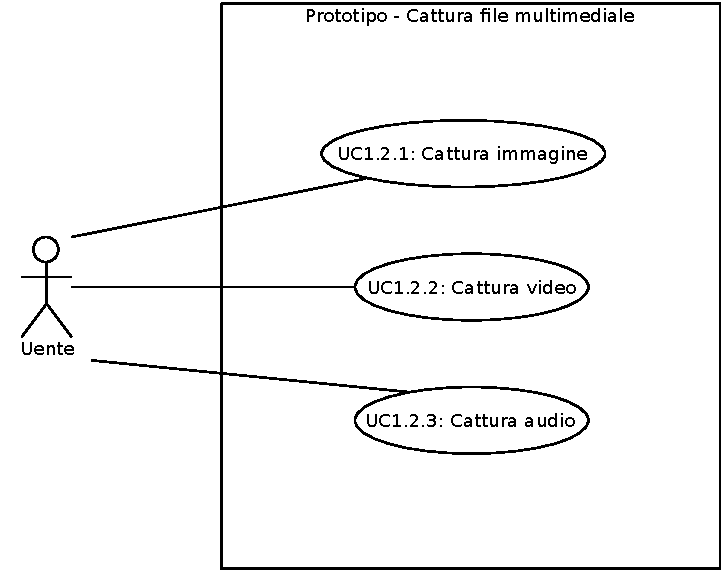
\includegraphics[scale=0.6]{gfx/useCase/UC1-2_Cattura_file_multimediale.pdf}
\caption{Caso d'uso UC1.2: Cattura file multimediale}
\label{fig:UC1.2}
\end{figure}

\begin{description}
\item[attori:] Utente;
\item[scopo e descrizione:] L'utente ha scelto l'opzione di cattura di dati multimediali e può decidere quale tipo di file catturare: immagine, audio o video;
\item[precondizione:] Il sistema mostra le possibili scelte all'utente;
\item[flusso principale degli eventi:] \hfill 
	\begin{enumerate}
	\item L'utente può catturare un'immagine;
	\item L'utente può catturare un video;
	\item L'utente può catturare un file audio;
	\end{enumerate}
\item[postcondizione:] Il sistema è pronto per la cattura del file multimediale prescelto.
\end{description}

\subsubsection{Caso d'uso UC1.2.1: Cattura immagine}
\begin{figure}[htb]
\centering
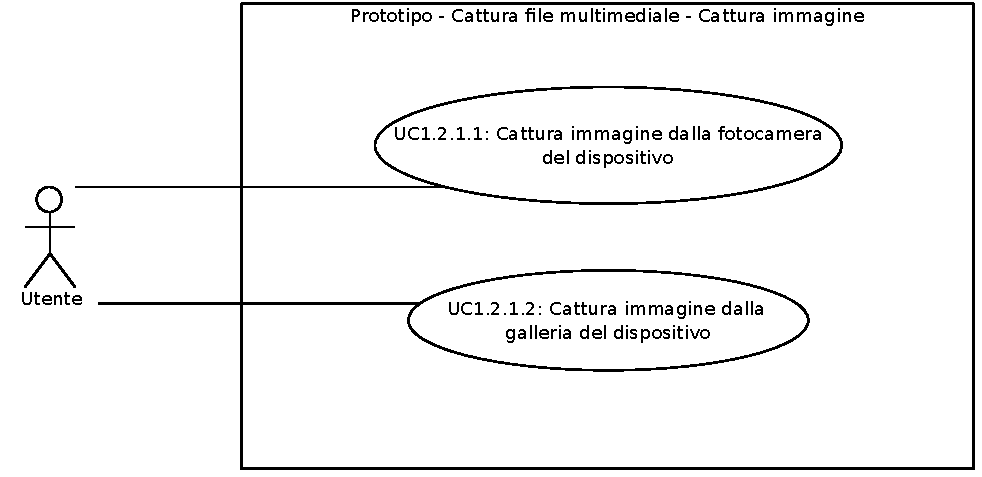
\includegraphics[scale=0.6]{gfx/useCase/UC1-2-1_Cattura_immagine.pdf}
\caption{Caso d'uso UC1.2.1: Cattura immagine}
\label{fig:UC1.2.1}
\end{figure}

\begin{description}
\item[attori:] Utente;
\item[scopo e descrizione:] L'utente ha scelto l'opzione di cattura di un'immagine e può scegliere se utilizzare la fotocamera del dispositivo oppure la galleria dello stesso;
\item[precondizione:] Il sistema mostra le possibili scelte all'utente;
\item[flusso principale degli eventi:] \hfill 
	\begin{enumerate}
	\item L'utente può catturare un'immagine dalla fotocamera del dispositivo;
	\item L'utente può catturare un'immagine dalla galleria del dispositivo;
	\end{enumerate}
\item[postcondizione:] Il sistema è pronto per la cattura dell'immagine dalla fonte prescelta.
\end{description}

\subsubsection{Caso d'uso UC1.2.1.1: Cattura immagine dalla fotocamera del dispositivo}
\begin{description}
\item[attori:] Utente;
\item[scopo e descrizione:] L'utente ha scelto la cattura di un'immagine dalla fotocamera del dispositivo;
\item[precondizione:] Il sistema è pronto per la cattura di una nuova immagine dalla fotocamera;
\item[scenari alternativi:] \hfill 
	\begin{enumerate}
	\item L'utente decide di annullare l'operazione di cattura; il sistema torna allo stato precedente la scelta dell'utente;
	\end{enumerate}
\item[postcondizione:] Il sistema ha catturato una nuova immagine e procede con il salvataggio.
\end{description}

\subsubsection{Caso d'uso UC1.2.1.2: Cattura immagine dalla galleria del dispositivo}
\begin{description}
\item[attori:] Utente;
\item[scopo e descrizione:] L'utente ha scelto la cattura di un'immagine dalla galleria del dispositivo;
\item[precondizione:] Il sistema è pronto per la cattura di una nuova immagine dalla galleria;
\item[scenari alternativi:] \hfill 
	\begin{enumerate}
	\item L'utente decide di annullare l'operazione di cattura; il sistema torna allo stato precedente la scelta dell'utente;
	\end{enumerate}
\item[postcondizione:] Il sistema ha catturato una nuova immagine e procede con il salvataggio.
\end{description}

\subsubsection{Caso d'uso UC1.2.2: Cattura video}
\begin{description}
\item[attori:] Utente;
\item[scopo e descrizione:] L'utente ha scelto la cattura di un video;
\item[precondizione:] Il sistema è pronto per la cattura di un nuovo video;
\item[scenari alternativi:] \hfill 
	\begin{enumerate}
	\item L'utente decide di annullare l'operazione di cattura; il sistema torna allo stato precedente la scelta dell'utente;
	\end{enumerate}
\item[postcondizione:] Il sistema ha catturato una nuovo video e procede con il salvataggio.
\end{description}

\subsubsection{Caso d'uso UC1.2.3: Cattura audio}
\begin{description}
\item[attori:] Utente;
\item[scopo e descrizione:] L'utente ha scelto la cattura di un file audio;
\item[precondizione:] Il sistema è pronto per la cattura di una nuovo file audio;
\item[scenari alternativi:] \hfill 
	\begin{enumerate}
	\item L'utente decide di annullare l'operazione di cattura; il sistema torna allo stato precedente la scelta dell'utente;
	\end{enumerate}
\item[postcondizione:] Il sistema ha catturato una nuovo file audio e procede con il salvataggio.
\end{description}

\subsubsection{Caso d'uso UC1.3: Recupero informazioni dispositivo}
\begin{description}
\item[attori:] Utente;
\item[scopo e descrizione:] L'utente ha scelto il recupero delle informazioni proprie del dispositivo;
\item[precondizione:] Il sistema è pronto per il recupero delle informazioni;
\item[postcondizione:] Il sistema ha recuperato le informazioni e procede con il salvataggio e la visualizzazione.
\end{description}

\subsubsection{Caso d'uso UC1.4: Recupero posizione corrente}
\begin{description}
\item[attori:] Utente,
\item[scopo e descrizione:] L'utente ha scelto il recupero della posizione corrente tramite il \ac{GPS} del dispositivo;
\item[precondizione:] Il sistema è pronto per il recupero della posizione;
\item[postcondizione:] Il sistema ha recuperato la posizione del dispositivo e procede con il salvataggio e la visualizzazione.
\end{description}

\subsubsection{Caso d'uso UC1.5: Lettura contatti dispositivo}
\begin{description}
\item[attori:] Utente;
\item[scopo e descrizione:] L'utente ha scelto la lettura dei contatti dal dispositivo;
\item[precondizione:] Il sistema è pronto per la lettura dei contatti presenti nel dispositivo;
\item[postcondizione:] Il sistema ha recuperato i contatti del dispositivo e procede con il salvataggio e la visualizzazione.
\end{description}

\subsubsection{Caso d'uso UC1.6: Gestione informazioni personali utente}
\begin{figure}[htb]
\centering
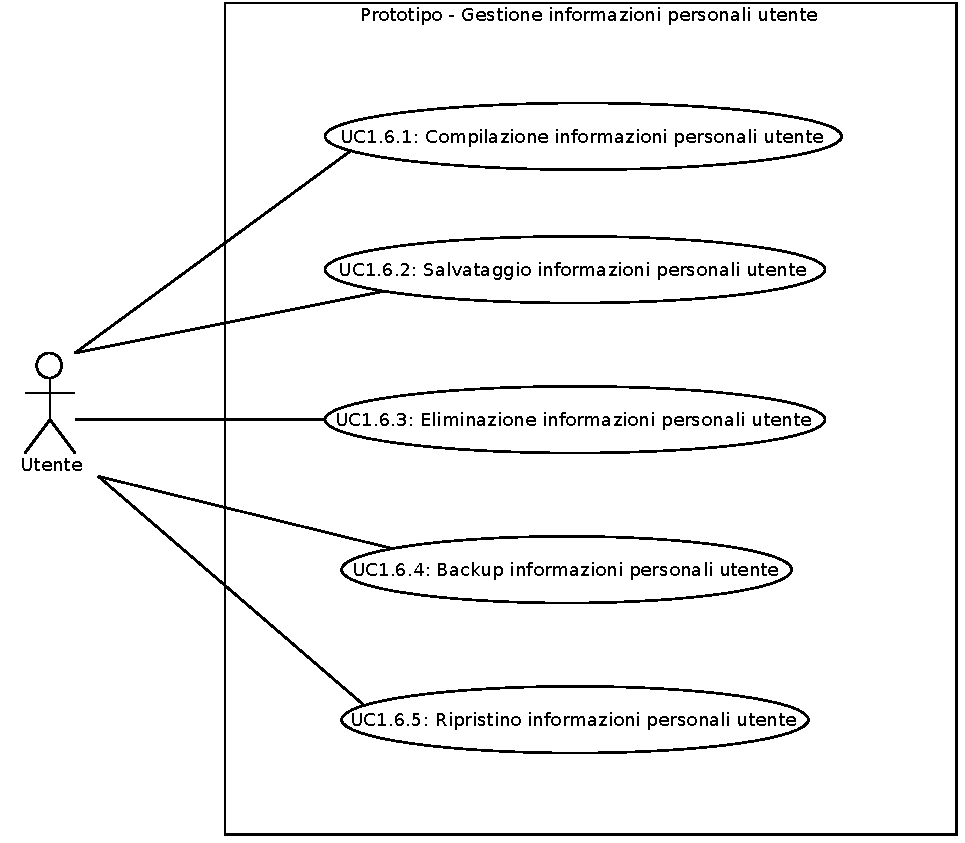
\includegraphics[scale=0.6]{gfx/useCase/UC1-6_Gestione_informazioni_personali_utente.pdf}
\caption{Caso d'uso UC1.6: Gestione informazioni personali utente}
\label{fig:UC1.6}
\end{figure}

\begin{description}
\item[attori:] Utente;
\item[scopo e descrizione:] L'utente ha scelto la gestione delle informazioni personali e può procedere con la compilazione di tali informazioni oppure salvare, eliminare, effettuare un backup o un ripristino di tali dati;
\item[precondizione:] Il sistema è pronto per gestire le informazioni personali dell'utente;
\item[flusso principale degli eventi:] \hfill
	\begin{enumerate}
	\item L'utente può compilare le informazioni personali;
	\item L'utente può salvare le informazioni personali;
	\item L'utente può eliminare le informazioni personali;
	\item L'utente può effettuare un backup delle informazioni personali;
	\item L'utente può effettuare un ripristino delle informazioni personali;
	\end{enumerate}
\item[postcondizione:] Il sistema è pronto ad eseguire l'opzione scelta dell'utente;
\end{description}

\subsubsection{Caso d'uso UC1.6.1: Compilazione informazioni personali utente}
\begin{description}
\item[attori:] Utente;
\item[scopo e descrizione:] L'utente ha scelto di compilare le informazioni personali;
\item[precondizione:] Il sistema è pronto per accettare l'immissione delle informazioni dell'utente;
\item[postcondizione:] Il sistema ha scritto le informazioni immesse dall'utente.
\end{description}

\subsubsection{Caso d'uso UC1.6.2: Salvataggio informazioni personali utente}
\begin{description}
\item[attori:] Utente;
\item[scopo e descrizione:] L'utente ha scelto di salvare le informazioni personali immesse;
\item[precondizione:] Il sistema è in possesso delle informazioni immesse dall'utente;
\item[postcondizione:] Il sistema ha salvato le informazioni immesse dall'utente.
\end{description}

\subsubsection{Caso d'uso UC1.6.3: Eliminazione informazioni personali utente}
\begin{description}
\item[attori:] Utente;
\item[scopo e descrizione:] L'utente ha scelto di eliminare le informazioni salvate;
\item[precondizione:] Il sistema possiede le informazioni dell'utente ed è pronto ad eliminarle;
\item[postcondizione:] Il sistema ha eliminato le informazioni dell'utente.
\end{description}

\subsubsection{Caso d'uso UC1.6.4: Backup informazioni personali utente}
\begin{description}
\item[attori:] Utente;
\item[scopo e descrizione:] L'utente ha scelto di effettuare un backup delle informazioni salvate;
\item[precondizione:] Il sistema possiede le informazioni salvate dell'utente ed è pronto al backup;
\item[postcondizione:] Il sistema ha effettuato il backup delle informazioni sulla memoria del dispositivo.
\end{description}

\subsubsection{Caso d'uso UC1.6.5: Ripristino informazioni personali utente}
\begin{description}
\item[attori:] Utente;
\item[scopo e descrizione:] L'utente ha scelto di ripristinare le informazioni di cui ha effettuato una copia di backup;
\item[precondizione:] Il sistema è pronto a ripristinare le informazioni dell'utente;
\item[postcondizione:] Il sistema a ripristinato le informazioni dell'utente.
\end{description}

\subsubsection{Caso d'uso UC1.7: Consultazione galleria immagini}
\begin{description}
\item[attori:] Utente;
\item[scopo e descrizione:] L'utente ha scelto di consultare la galleria delle immagini;
\item[precondizione:] Il sistema è pronto a visualizzare la galleria delle immagini;
\item[postcondizione:] Il sistema ha visualizzato la galleria delle immagini.
\end{description}

\subsubsection{Caso d'uso UC1.8: Consultazione libreria audio/video}
\begin{description}
\item[attori:] Utente;
\item[scopo e descrizione:] L'utente ha scelto di consultare la libreria audio/video;
\item[precondizione:] Il sistema è pronto a visualizzare la libreria audio/video;
\item[postcondizione:] Il sistema ha visualizzato la libreria audio/video.
\end{description}

\subsubsection{Caso d'uso UC1.9: Visualizzazione dato acquisito}
\begin{description}
\item[attori:] Sistema;
\item[scopo e descrizione:] Il sistema visualizza il dato acquisito;
\item[precondizione:] Il sistema è pronto a visualizzare il dato acquisito;
\item[postcondizione:] Il sistema ha visualizzato il dato acquisito.
\end{description}

\subsubsection{Caso d'uso UC1.10: Salvataggio dato acquisito}
\begin{description}
\item[attori:] Sistema;
\item[scopo e descrizione:] Il sistema salva il dato acquisito;
\item[precondizione:] Il sistema è pronto a visualizzare il dato acquisito;
\item[postcondizione:] Il sistema ha salvato il dato acquisito.
\end{description}

\newpage
\subsection{Requisiti}
Vengono ora descritti i requisiti suddivisi per tipologia.

\subsubsection{Requisiti funzionali}
Di seguito viene riportata la tabella che esprime i requisiti funzionali.
%**************************************
%    tabella requisiti funzionali
%**************************************
\begin{longtable}{cp{0.7\textwidth}c}
\caption{Tabella dei requisiti funzionali}
\label{tab:requsiti funzionali} \\
%intestazione iniziale
\toprule
Codice & Descrizione & Fonte \\
\midrule
\endfirsthead
%intestazione normale
\multicolumn{3}{l}{\footnotesize\itshape Continua dalla pagina precedente}\\
\toprule
Codice & Descrizione & Fonte \\
\midrule
\endhead
%piede normale
\midrule
\multicolumn{3}{r}{\footnotesize\itshape Continua nella prossima pagina}\\
\endfoot
%piede finale
\bottomrule
\multicolumn{3}{r}{\footnotesize\itshape Si conclude dalla pagina precedente}\\
\endlastfoot
%corpo della tabella
%TODO aggiungere funzioni di prodotto
R1F1
& L'utente deve poter scegliere l'opzione di lettura barcode
& UC1.1 \\
\midrule
\multirow{6}*{R1F2}
& \multirow{6}*{\parbox{0.7\textwidth}{L'utente deve poter scegliere l'opzione di cattura di un file multimediale}}
& UC1.2 \\
& & UC1.2.1 \\
& & UC1.2.1.1 \\
& & UC1.2.1.2 \\
& & UC1.2.2 \\
& & UC1.2.3 \\
\midrule
\multirow{3}*{R1F2.1}
& \multirow{3}*{\parbox{0.7\textwidth}{L'utente deve poter scegliere l'opzione di cattura di un'immagine}}
& UC1.2.1 \\
& & UC1.2.1.1 \\
& & UC1.2.1.2 \\
\midrule
R1F2.2
& L'utente deve poter scegliere l'opzione di cattura di un video
& UC1.2.2 \\
\midrule
R1F2.3
& L'utente deve poter scegliere l'opzione di cattura di un file audio
& UC1.2.3 \\
\midrule
R1F3
& L'utente deve poter scegliere l'opzione di recupero delle informazioni del dispositivo
& UC1.3 \\
\midrule
R1F4
& L'utente deve poter scegliere l'opzione di recupero della posizione corrente
& UC1.4 \\
\midrule
R1F5
& L'utente deve poter scegliere l'opzione di lettura dei contatti del dispositivo
& UC1.5 \\
\midrule
\multirow{6}*{R1F6}
& \multirow{6}*{\parbox{0.7\textwidth}{L'utente deve poter scegliere l'opzione di gestione delle informazioni personali}}
& UC1.6 \\
& & UC1.6.1 \\
& & UC1.6.2 \\
& & UC1.6.3 \\
& & UC1.6.4 \\
& & UC1.6.5 \\
\midrule
R1F6.1
& L'utente deve poter scegliere di compilare le informazioni personali
& UC1.6.1 \\
\midrule
R1F6.2
& L'utente deve poter scegliere di salvare le informazioni personali
& UC1.6.2 \\
\midrule
R1F6.3
& L'utente deve poter scegliere di eliminare le informazioni personali
& UC1.6.3 \\
\midrule
R1F6.4
& L'utente deve poter scegliere di effettuare il backup delle informazioni personali
& UC1.6.4 \\
\midrule
R1F6.5
& L'utente deve poter scegliere di effettuare il ripristino delle informazioni personali
& UC1.6.5 \\
\midrule
R1F7
& L'utente deve poter scegliere di consultare la galleria immagini
& UC1.7 \\
\midrule
R1F8
& L'utente deve poter scegliere di consultare la libreria audio/video
& UC1.8 \\
\midrule
R1F9
& Il sistema deve visualizzare i dati non appena vengono acquisiti
& UC1.9 \\
\midrule
R1F10
& Il sistema deve salvare i dati non appena vengono acquisiti
& UC1.10 \\
\end{longtable}

\subsubsection{Requisiti di vincolo}
Di seguito viene riportata la tabella che esprime i requisiti di vincolo.
%**************************************
%    tabella requisiti di vincolo
%**************************************
\begin{longtable}{cp{0.7\textwidth}c}
\caption{Tabella dei requisiti di vincolo}
\label{tab:requsiti vincolo} \\
%intestazione iniziale
\toprule
Codice & Descrizione & Fonte \\
\midrule
\endfirsthead
%intestazione normale
\multicolumn{3}{l}{\footnotesize\itshape Continua dalla pagina precedente}\\
\toprule
Codice & Descrizione & Fonte \\
\midrule
\endhead
%piede normale
\midrule
\multicolumn{3}{r}{\footnotesize\itshape Continua nella prossima pagina}\\
\endfoot
%piede finale
\bottomrule
\multicolumn{3}{r}{\footnotesize\itshape Si conclude dalla pagina precedente}\\
\endlastfoot
%corpo della tabella
R
\end{longtable}

%\subsection{Requisiti prestazionali}
%Di seguito viene riportata la tabella che esprime i requisiti prestazionali.
%%**************************************
%    tabella requisiti prestazionali
%**************************************

\subsubsection{Requisiti di qualità}
Di seguito viene riportata la tabella che esprime i requisiti di qualità.
%**************************************
%    tabella requisiti di qualità
%**************************************
\rowcolors{1}{lightCyan}{paleTurquoise}
\begin{longtable}{lp{0.60\textwidth}l}
\hiderowcolors
\caption{Requisiti di qualità -- SensorDevice}
\label{tab:requsiti qualità} \\
%intestazione iniziale
\toprule \hiderowcolors
Codice & Descrizione & Fonte \\
\midrule
\endfirsthead
%intestazione normale
\hiderowcolors
\multicolumn{3}{l}{\footnotesize\itshape Continua dalla pagina precedente}\\
\toprule \hiderowcolors
Codice & Descrizione & Fonte \\
\midrule
\endhead
%piede normale
\midrule \hiderowcolors
\multicolumn{3}{r}{\footnotesize\itshape Continua nella prossima pagina}\\
\endfoot
%piede finale
\bottomrule %\hiderowcolors
%\multicolumn{3}{r}{\footnotesize\itshape Si conclude dalla pagina precedente}\\
\endlastfoot
%corpo della tabella
\showrowcolors
R0Q1 & Deve essere prodotta la documentazione del codice sorgente dell'applicazione 	& Capitolato \\[7mm]
R0Q2 & Deve essere prodotto un resoconto dettagliato delle funzionalità implementate	& Capitolato \\
\end{longtable}